\section{Resolution of measurement}
%The position of a detected particle is known to within a specified distance, which translates into a resolution in the measurement of the opening angle between a pair of particles.
A particle's reconstructed position along a detector's length has an error of $\pm$13 cm.
There is also a position uncertainty of $\pm 7.5$ cm along the axis of each detector's 15 cm width.
The uncertainty in n-n opening angle determination is quantified by propagating the uncertainties in the positions of each detected neutron through the formula for the calculation of opening angle, which is
\begin{displaymath}
    \theta_{nn} = \text{arccos}\left(\frac{\vec{v_{1}}^{\,}\cdot\vec{v_{2}}^{\,}}{|\vec{v_{1}}^{\,}||\vec{v_{2}}^{\,}|}\right)
\end{displaymath}
where $\vec{v_{1}}^{\,} = (x_1,y_1,z_1)$ and $\vec{v_{2}}^{\,} = (x_2,y_2,z_2)$ are the detected positions of the two neutrons.
The propagation of error through this formula is achieved by evaluating the following expression
\begin{eqnarray}
\label{eq:propagation}
 \Delta \theta_{nn} & = & \left( \left(\Delta x_1 \frac{\partial \theta}{\partial x_1}\right)^{2} + \left(\Delta y_1 \frac{\partial \theta}{\partial y_1}\right)^{2} + \left(\Delta z_1 \frac{\partial \theta}{\partial z_1}\right)^{2} + \right. \\
 & & \left. + \left(\Delta x_2 \frac{\partial \theta}{\partial x_2}\right)^{2} + \left(\Delta y_2\frac{\partial \theta}{\partial y_2}\right)^{2} + \left(\Delta z_2 \frac{\partial \theta}{\partial z_2}\right)^{2} \right) ^{\frac{1}{2}} \, ,  \nonumber
\end{eqnarray}
where the $\Delta$'s represent the uncertainty in the variable that directly follows each $\Delta$.
In Fig.~\ref{fig:OpeningAngleRes}, all events in each opening angle bin are fed through Eq. \ref{eq:propagation}, and the results for each bin are averaged.
Fig.~\ref{fig:OpeningAngleRes} can be interpreted as the opening angle resolution as a function of $\theta_{nn}$.
\begin{figure}[h]
    \centering
    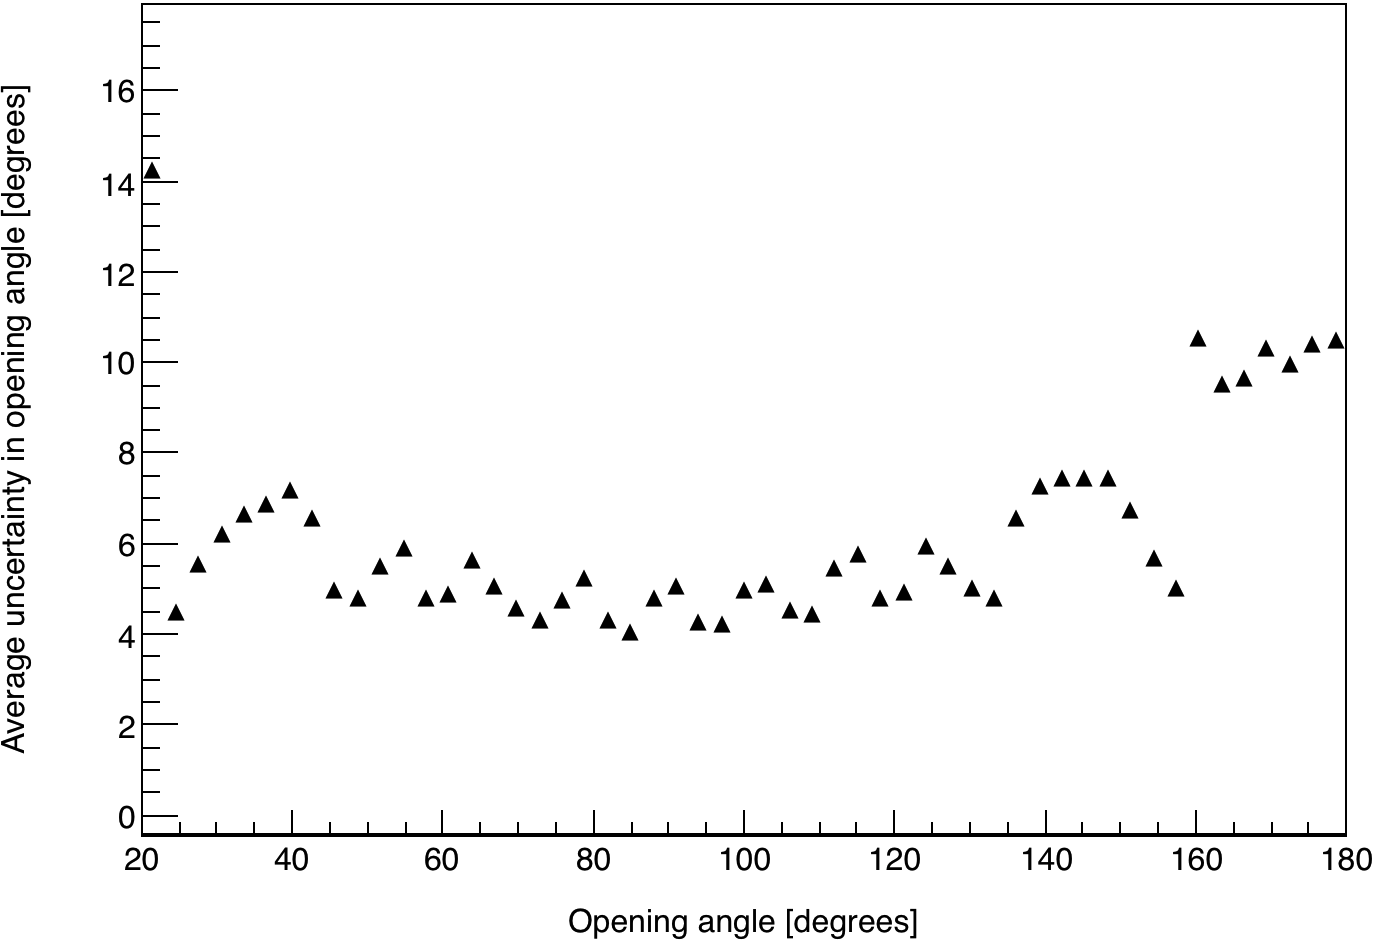
\includegraphics[width = 0.85\textwidth]{Content/Errors/OpeningAngleUncertainty.png}
    \caption{Uncertainties in opening angle determined from the propagation of position uncertainties through the opening angle calculation.
     %The uncertainty of a given opening angle measurement depends on which detectors are involved and the position of the particles on the detectors.
    % For this reason, the uncertainty of measurements falling within each angle bin is a distribution, so the average uncertainties are plotted here.
    The y-axis can be viewed as a measure of angular resolution in the sense that it represents the smallest angular difference that can be considered statistically significant.
    }
    \label{fig:OpeningAngleRes}
\end{figure}

\section{Counting error}
The uncertainty in the number of observed events is always assumed to be equal to $\sqrt{N}$, as per Poissonian  statistics, where N is the number of observed events.
This value is then propagated through the analysis procedure using the standard methods for the propagation of error.
The vertical error bars seen in all results are due solely to such counting error.

\FloatBarrier

